\chapter{SNAP}

Esta clase tiene como objetivo familiarizarnos con la interpretación visual de imágenes SAR en las bandas L, C y X. Para esto se estudiaran las interacciones con distintos blancos para cada una de las bandas.

\section{Banda-X}

Las imágenes adquiridas en \emph{Banda X} son las que tienen menor longitud de onda. Serán por lo tanto las que menos penetración tengan en la vegetación y las que más componente de backscatter presenten en suelos sin cobertura (Figura \ref{fig:bandaX}).

\begin{figure}[h!]
    \centering
    %\includegraphics{fig:bandaX}
    \caption{Interacciónes con distintos blancos: -a- superficial, -b- subsuperficial, -c- doble rebote y -d- en volumen.}
    \label{bandaX}
\end{figure}

Abra la imagen \path{CSKS3_GEC_B_S2_03_HH_RD_SF_20141221211655_20141221211703.h5} de la carpeta \path{material/raster_data/COSMO}. Despliege la banda \emph{Sigma\_HH_db}.

Observe guiandose con el mapa de la zona (Figura \ref{fig:mapa})
\begin{itemize}
    \item La zona de la pista de aterrizaje se observa de color obscuro.
    \item Las zonas urbanas se observan en colores brillantes.
    \item Las laderas de las montañas con bosque se ven en colores brillantes.
    \item La montaña parece estar inclinada hacia la derecha.
\end{itemize}

\begin{figure}[h!]
    \centering
    %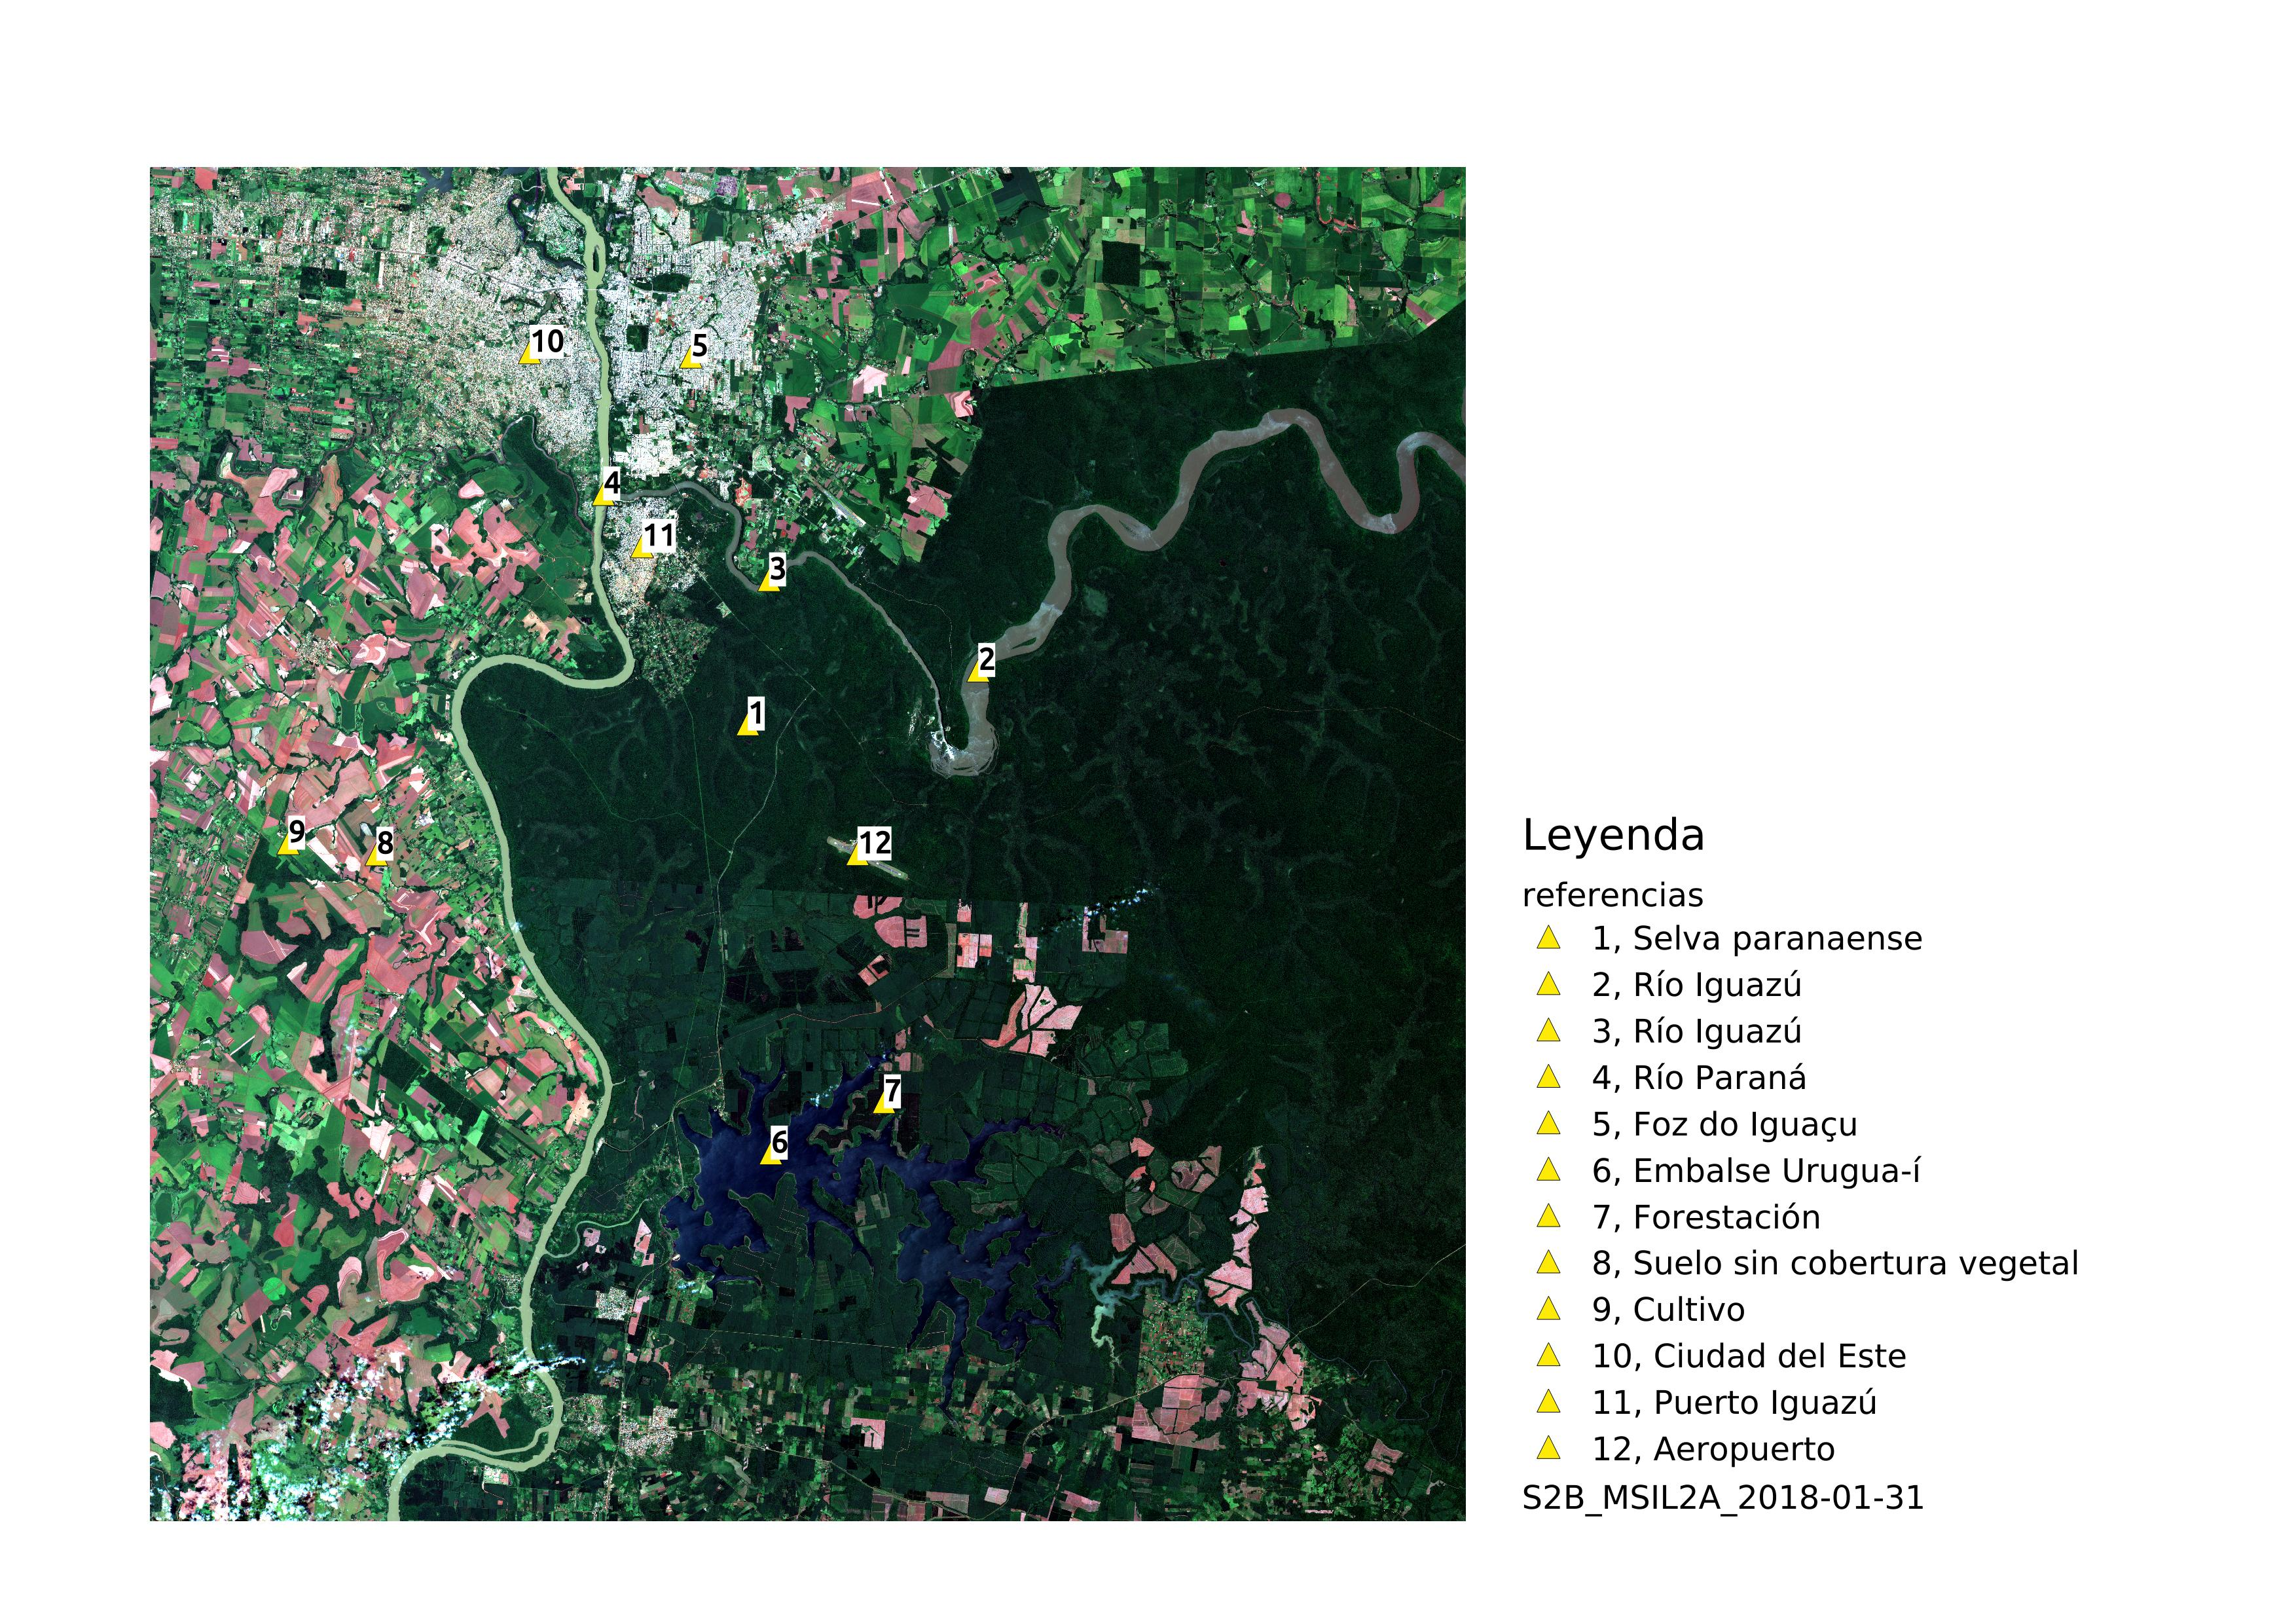
\includegraphics{fig:mapa.png}
    \caption{Mapa de la zona de interés. Se observa el aeropuerto de Ushuahia, la ciudad de Ushuahia, zonas boscosas, con agua y montañas con distintoas}
    \label{fig:mapa}
\end{figure}

\begin{que}
    ¿Que le permite decir sobre las ciudades el hecho que la reflectancia sea máxima en dicha zona?
\end{que}

\begin{que}
    ¿Que puede decir sobre la pista de aterrizaje?
\end{que}

\begin{que}
    ¿Le permite esta imagen separar las zonas con cobertura vegetal de las zonas sin cobertura?
\end{que}

\section{Banda C}

Las imágenes adquiridas en \emph{Banda C} son las que tienen longitudes de onda intermedias. Tendrán por lo tanto menos reflectancia en los suelos sin coberturaa y nos permitiran extraer información sobre el scattering en volumnes (Figura \ref{fig:bandaC}).

\begin{figure}[h!]
    \centering
    %\includegraphics{fig:bandaL}
    \caption{Interacciónes con distintos blancos: -a- superficial, -b- subsuperficial, -c- doble rebote y -d- en volumen.}
    \label{bandaC}
\end{figure}

Abra la imagen \path{SENTINEL} de la carpeta \path{material/raster_data/SENTINEL1}. Despliege la banda \emph{Sigma\_HH_db}.

Observe guiandose con el mapa de la zona (Figura \ref{fig:mapa})
\begin{itemize}
    \item
\end{itemize}

\section{Banda L}

Las imágenes adquiridas en \emph{Banda L} son las que tienen mayor longitud de onda. Tendran en general interacciones especulares con los suelos sin cobertura, pero una buena longitud de penetración en la superficie. Además permitirán identificar propiedades de las coberturas vegetadas por debajo del canopeo (Figura \ref{fig:bandaL}).

\begin{figure}[h!]
    \centering
    %\includegraphics{fig:bandaL}
    \caption{Interacciónes con distintos blancos: -a- superficial, -b- subsuperficial, -c- doble rebote y -d- en volumen.}
    \label{bandaL}
\end{figure}

Abra la imagen \path{ALOS} de la carpeta \path{material/raster_data/ALOS}. Despliege la banda \emph{Sigma\_HH_db}.

Observe guiandose con el mapa de la zona (Figura \ref{fig:mapa})
\begin{itemize}
    \item
\end{itemize}

\section{Actividad}

Comparando las tres imágenes SAR utilizadas responda

\begin{que}
    ¿Que coberturas tienen siempre valores altos de brillo? ¿Como se puede interpretar geometricamente?
\end{que}

\begin{que}
    ¿Que coberturas tienen siempre valores bajos de brillo? ¿Como se puede interpretar geometricamente?
\end{que}

\begin{que}
    ¿Cual es la cobertura que más cambian al cambiar de una banda a otra?
\end{que}

\begin{que}
    ¿Cuales son las coberturas con más ruido dentro de las imágenes?
\end{que}

\begin{que}
    Observe las imágenes que no se encuentran en dB. ¿Que diferencia encuentra en la distribución de valores de brillo?
\end{que}

\begin{que}
    Observe el histograma de las imagenes en intensidad y dB\footnote{Analylis, Histogram}. ¿Como se comparan las distribuciones? ¿Cual le parece le permite distinguir más detalles en la imagen?
\end{que}
